\FloatBarrier
\section{CP violation sensitivity}
\label{sec:cp_sens}

In this section, CPV sensitivity results are presented. For simplicity, only true normal ordering will be shown unless explicitly stated. In all cases, a joint ND+FD fit is performed, and a $\theta_{13}$ penalty is always applied, as described in Section~\ref{sec:analysis_framework}. The Asimov sensitivities as shown in Section~\ref{sec:run_plan_opt} are informative, but do not give information on how the expected sensitivity may vary with statistical or systematic uncertainties. Or for variations in the other oscillation parameters of interest. In this section, the toy throwing approach described in Section~\ref{sec:analysis_framework} is used to explore the CPV sensitivity in more detail.

\begin{figure}[htbp]
  \centering
  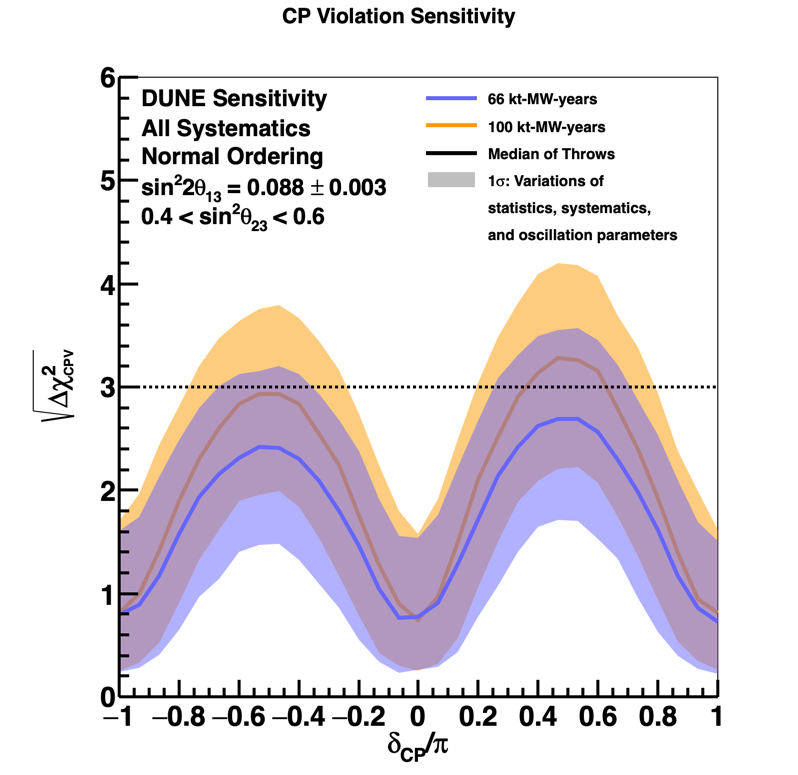
\includegraphics[width=0.8\linewidth, trim={0cm 0cm 0cm 2.3cm}, clip]{cpv_two_exps_throws_nh_2019_v4_lowexp.png}\\
  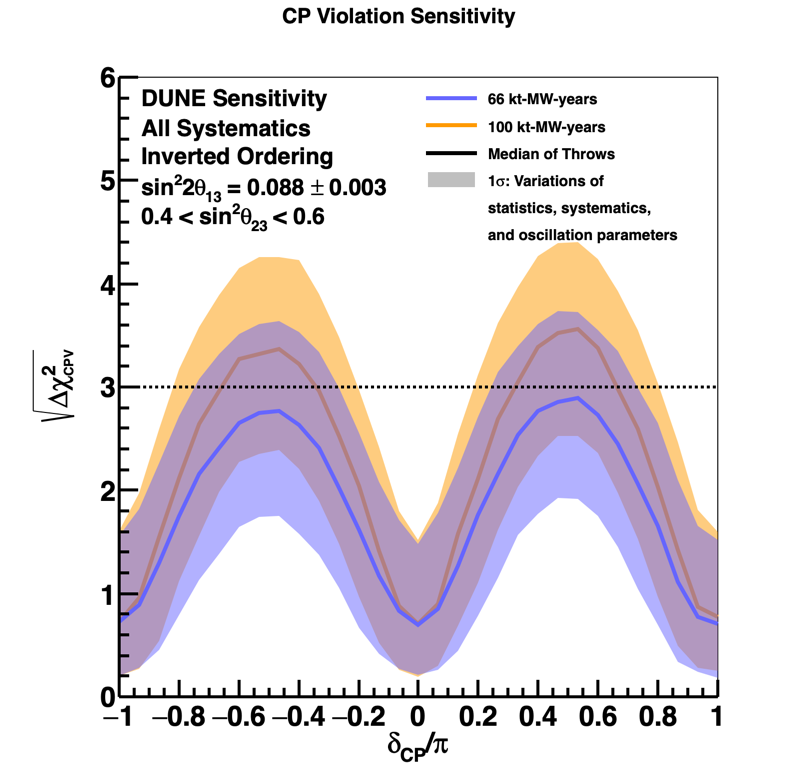
\includegraphics[width=0.8\linewidth, trim={0cm 0cm 0cm 2.3cm}, clip]{cpv_two_exps_throws_ih_2019_v4_lowexp.png}
  \caption{Significance of the DUNE determination of CP-violation ($\deltacp \neq [0,\pm\pi]$) as a function of the true value of \deltacp, for 66 ktMWyr (blue) and 100 ktMWyr (orange) exposures, for normal (top) and inverted (bottom) orderings. The width of the transparent bands cover 68\% of fits in which random throws are used to simulate statistical variations and select true values of the oscillation and systematic uncertainty parameters, constrained by pre-fit uncertainties. The solid lines show the median sensitivity.}
  \label{fig:cpv_bands}
\end{figure}
Figure~\ref{fig:cpv_bands} shows the significance with which \dword{cpv} ($\deltacp \neq [0, \pm\pi]$) can be observed for both \dword{no} \dword{io}, for exposures of 66 kTMWyr and 100 ktMWyr. For each throw of the systematic, other oscillation parameters and statistics, two fits are carried out, one where the \deltacp is fixed at CP-conserving values, and another where it is allowed to vary. The difference in the best-fit $\chi^{2}$ values is calculated:
\begin{equation}
  \Delta\chi^{2} = \chi^{2}_{0,\pm\pi} - \chi^{2}_{\mathrm{CPV}},
  \label{eq:cpv_chi2}
\end{equation}
\noindent and the square root of the difference is the significance shown on the y-axis of Figure~\ref{fig:cpv_bands}. We note that this constant-\dchisq method is valid as long as Wilks' can be applied~\cite{wilks}.

The sensitivity shown in Figure~\ref{fig:cpv_bands} has the characteristic double peak structure because the significance of a \dword{cpv} measurement decreases around CP-conserving values. The median sensitivity never reaches exactly zero at CP-conserving values due to the systematic and statistical throws. Median sensitivities are slightly higher for \dword{io} than for \dword{no}, and by exposures of 100 ktMWyr, the median sensitivity exceeds 3$\sigma$ for the maximal CP-violating values of $\pm\pi/2$. This presentation of the CPV sensitivity was followed in Ref.~\cite{Abi:2020qib}, and is very informative at high exposures. However at low exposures as shown in Figure~\ref{fig:cpv_bands}, the spread in the sensitivity is harder to interpret.

\begin{figure*}[htbp]
  \centering
  \subfloat[24 ktMWyr] {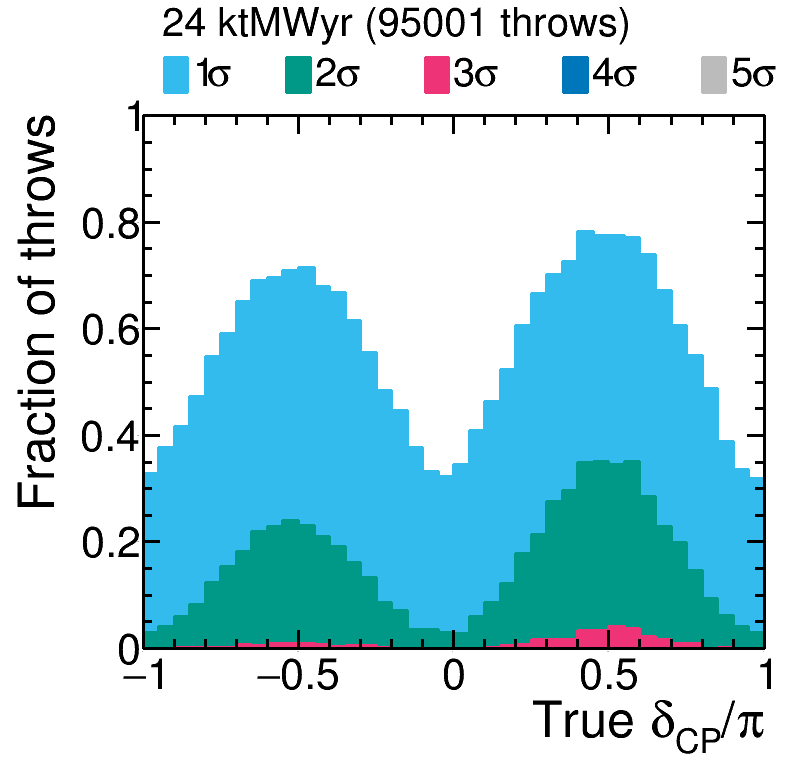
\includegraphics[width=0.33\linewidth]{cpv_throws_24ktMWyr_NH_th13.png}}
  \subfloat[66 ktMWyr] {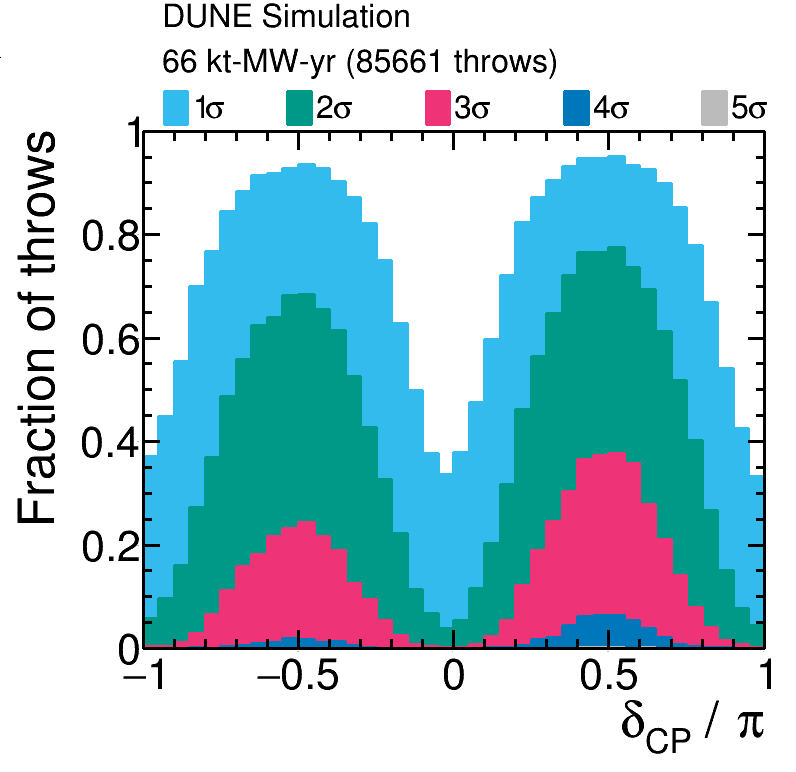
\includegraphics[width=0.33\linewidth]{cpv_throws_66ktMWyr_NH_th13.png}}
  \subfloat[100 ktMWyr]{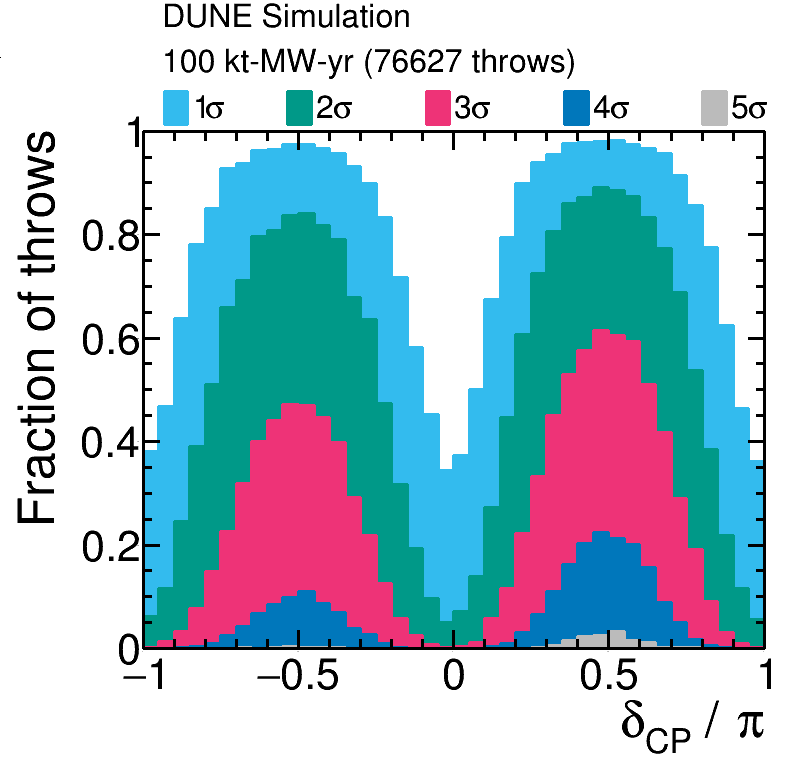
\includegraphics[width=0.33\linewidth]{cpv_throws_100ktMWyr_NH_th13.png}}\\
  \subfloat[150 ktMWyr]{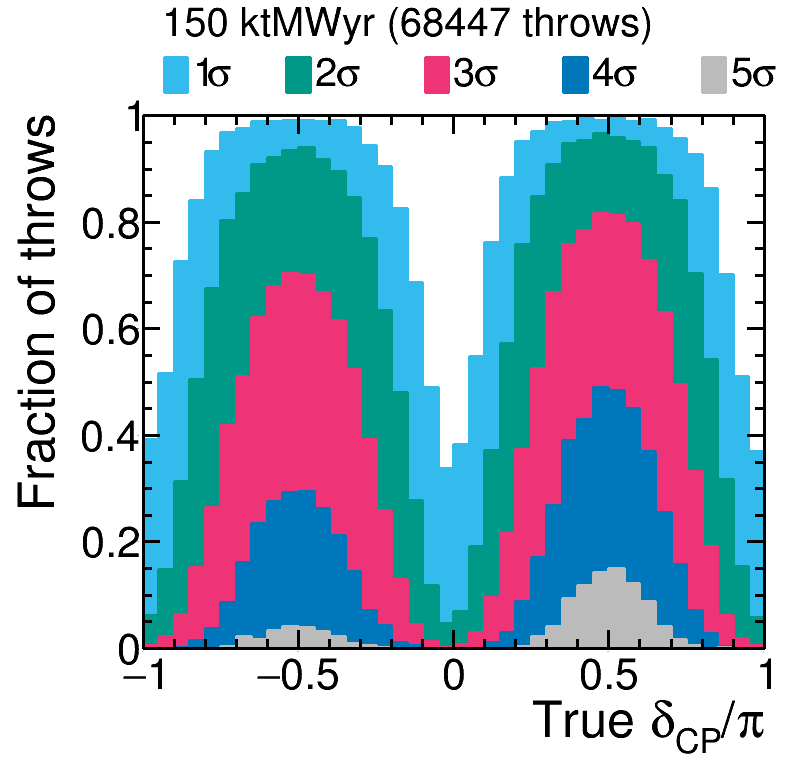
\includegraphics[width=0.33\linewidth]{cpv_throws_150ktMWyr_NH_th13.png}}
  \subfloat[197 ktMWyr]{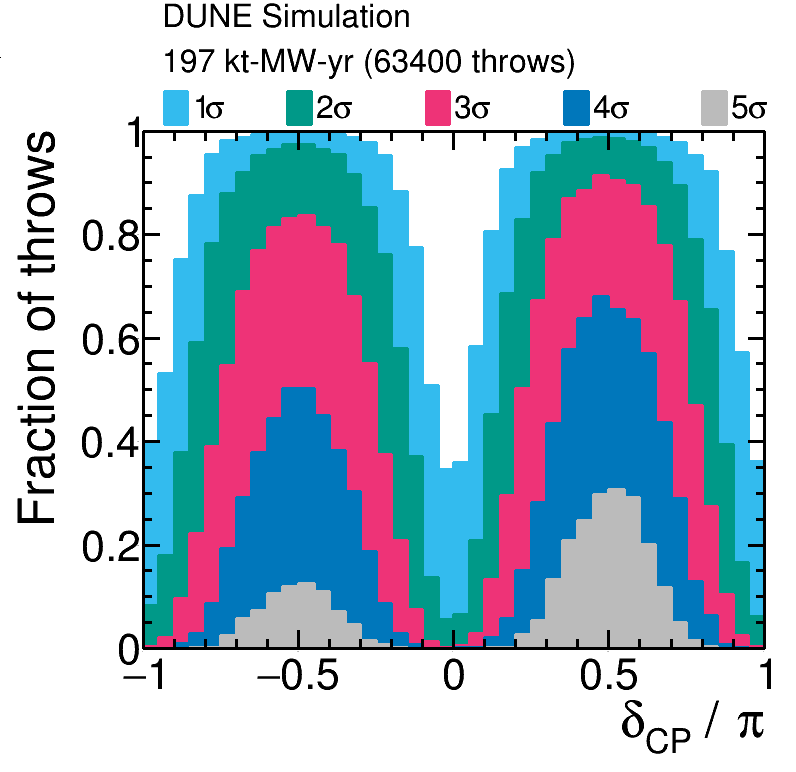
\includegraphics[width=0.33\linewidth]{cpv_throws_197ktMWyr_NH_th13.png}}
  \subfloat[334 ktMWyr]{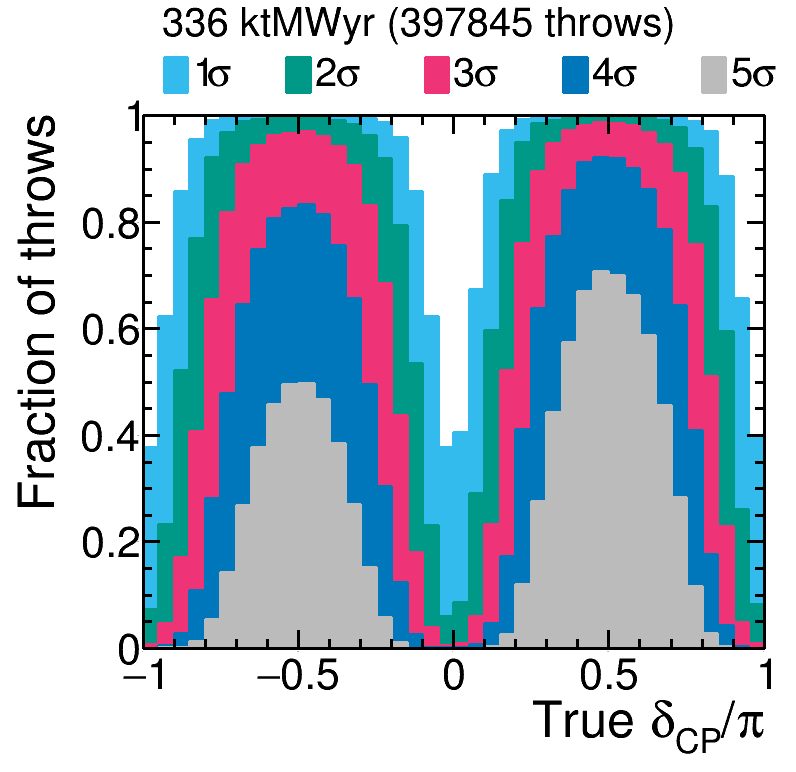
\includegraphics[width=0.33\linewidth]{cpv_throws_334ktMWyr_NH_th13.png}}
  \caption{Fraction of throws for which the DUNE sensitivity to CP-violation ($\deltacp \neq [0,\pm\pi]$) exceeds 1--5$\sigma$ significance, as a function of the true value of \deltacp. Shown for \dword{no}, for a number of different exposures. The number of throws used to make each figure is also shown.}
  \label{fig:cpv_over_time}
\end{figure*}
\begin{figure*}[htbp]
  \centering
  \subfloat[$\deltacp = -\pi/2$] {\includegraphics[width=0.8\columnwidth]{{fraction_throws_vs_exp_dcp-0.5}.pdf}}
  \subfloat[$\deltacp = +\pi/2$] {\includegraphics[width=0.8\columnwidth]{{fraction_throws_vs_exp_dcp0.5}.pdf}}
  \caption{Fraction of throws for which the DUNE sensitivity to CP-violation ($\deltacp \neq [0,\pm\pi]$) exceeds 1--5$\sigma$ significance, at $\deltacp = \pm\pi/2$, shown as a function of exposure, for \dword{no}.}
  \label{fig:cpv_vs_exp}
\end{figure*}
Figure~\ref{fig:cpv_over_time} provides an alternative way to present the results of the throws. The fraction of throws for which Equation~\ref{eq:cpv_chi2} exceeds different confidence values are shown, for 1--5$\sigma$ significances, for a variety of exposures. It shows the probability for DUNE to observe a significance above a discrete threshold, as a function of the true value of \deltacp. The point at which the median sensitivity (50\% of throws) passes different significance thresholds can be easily read from the figures, and can be compared with those shown in Figure~\ref{fig:cpv_bands}. Note that the highest exposure shown, 334 ktMWyr, is equivalent to the seven year exposure using the staging scenario from Ref.~\cite{Abi:2020qib}. The same double peak structure seen in Figure~\ref{fig:cpv_bands} can be observed. The median sensitivity to CPV exceeds 3$\sigma$ after $\sim$100 ktMWyr, but a significant fraction of throws exceed 3$\sigma$ at 66 ktMWyr. Likewise, although the median significance to CPV does not exceed 5$\sigma$ until $\sim$334 ktMWyr, there are significant fractions of throws at lower exposures which reach $5\sigma$ significance. This presentation also shows that by 334 ktMWyr exposures, the number of throws for which the significance is less than 3$\sigma$ at maximal values of \deltacp is very low. The number of throws used to generate the plots at each exposure is indicated on each plot. The number of throws decreases as a function of exposure because fixed computing resources were used for each configuration, and the time for the ensemble of fits carried out for each throw to complete increases slightly with exposure. The final 334 ktMWyr exposure has more throws because it was generated for the analysis presented in Ref.~\cite{Abi:2020qib}, where more than one projection was considered --- requiring more throws to sample the space.

Figure~\ref{fig:cpv_vs_exp} shows the fraction of throws which exceed different significance thresholds at the maximal \deltacp violation values of $\pm\pi/2$, as a function of exposure. Figure~\ref{fig:cpv_vs_exp} was produced using the same throws used for Figure~\ref{fig:cpv_over_time}, with additional points from higher exposures used in Ref.~\cite{Abi:2020qib}, but not shown in Figure~\ref{fig:cpv_over_time} (646 ktMWyr and 1104 ktMWyr). For \dword{no}, the significance at $\deltacp = +\pi/2$ is slightly stronger than at $\deltacp = -\pi/2$. For \dword{io}, the significance would be more similar between the two points, which can be observed from Figure~\ref{fig:cpv_bands}, but is not shown in Figures~\ref{fig:cpv_over_time} or~\ref{fig:cpv_vs_exp}.

% \FloatBarrier
% \subsection{Feldman-Cousins studies}
Previous results have been calculated confidence intervals and significances using constant $\Delta\chi^{2}$ critical values. For example, in the CPV results shown in Figure~\ref{fig:cpv_over_time}, the confidence intervals are calculated assuming one degree of freedom, so $\Delta\chi^{2} \leq 1, 4, 9$ corresponds to a significance of 1, 2 and 3$\sigma$. This assumption holds when Wilks' theorem can be applied~\cite{wilks}, but can lead to incorrect coverage where it cannot. This breaks down around physical boundaries, in the case of cyclic parameters, and where there are significant degeneracies. It is likely that a constant $\Delta\chi^{2}$ treatment will break down for \deltacp, where all of these issues apply, as has indeed been shown by T2K~\cite{Abe:2021gky}. The Feldman-Cousins method~\cite{Feldman:1997qc} is a brute force numerical method to calculate confidence intervals with correct coverage.

A large number of toy experiments are produced, where the parameter(s) of interest (here \deltacp) is set to the desired true value, all other systematic and oscillation parameters are thrown, as described in Section~\ref{sec:analysis_framework}, and a statistical throw is made, for the two ND samples and four FD sample used in the analysis. Then two fits are performed, one where the parameter(s) of interest is fixed to the true value, and another where is is allowed to vary. In both fits, all other parameters are allowed to vary. For each throw, a \dchisq is calculated using the minimum $\chi^{2}$ values for those two fits, as in Equation~\ref{dchisq_fc}.
\begin{equation}
  \Delta\chi^{2} = \chi^{2}(\theta_{\mathrm{true}}) - \min_{\theta}\chi^{2}(\theta)
  \label{eq:dchisq_fc}
\end{equation}
\begin{figure}[htbp]
  \centering
  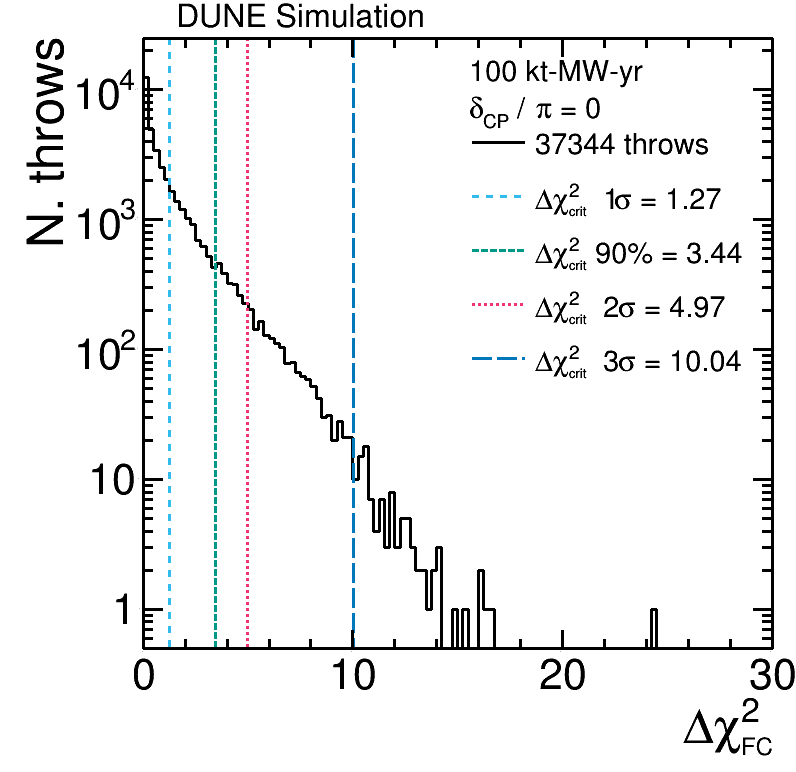
\includegraphics[width=0.8\columnwidth]{nh_FC_ndfd_100ktMWyr_dcp0.png}
  \caption{Distribution of \dchisq values, calculated using Equation~\ref{eq:dchisq_fc}, for a large number of throws with true $\deltacp = 0$, and a 100 ktMWyr exposure. The \dchisqcrit values (vertical lines) obtained using the Feldman-Cousins method show the \dchisq value below which 68.27\% (1$\sigma$), 90\%, 95.45\% (2$\sigma$) and 99.73\% (3$\sigma$) of throws reside, with the calculated values given in the legend. The number of throws used is also given.}
  \label{fig:fc_throws}
\end{figure}
The distribution of these throws is used to calculate the \dchisqcrit that gives the desired coverage, with the appropriate fraction of toys above/below the calculated value. A distribution of \dchisq values is shown in Figure~\ref{fig:fc_throws} for an example ND+FD analysis with a 100ktMWyr exposure at the far detector, equal FHC and RHC run fractions, and with a $\theta_{13}$ penalty applied. In Figure~\ref{fig:fc_throws}, the \dchisqcrit values corresponding to for 68.27\% (1$\sigma$), 90\%, 95.45\% (2$\sigma$) and 99.73\% (3$\sigma$) of the throws are indicated. The \dchisqcrit values were only calculated up to the 3$\sigma$ level due to the very large number of throws required for higher confidence levels.

An uncertainty on the value of \dchisqcrit obtained from the toy throw distribution (e.g., Figure~\ref{fig:fc_throws}), is obtained using a bootstrap rethrowing method~\cite{rice2006mathematical}. The empirical PDF obtained from the throws is treated as the true PDF, and $B$ independent samples of size $n$ are drawn from it, where $n$ is the total number of throws used to build the empirical PDF. Note that each throw can be drawn multiple times in this method. Then, the standard deviation $s_{\hat{\vartheta}}$, on the \dchisqcrit values of interest, $\vartheta$, are calculated for each of the $B$ samples using:
\begin{equation}
  s_{\hat{\vartheta}} = \sqrt{\frac{1}{B} \sum^{B}_{i=0} (\vartheta_{i}^{*} - \bar{\vartheta}^{*})^{2}},
  \label{eq:fc_uncertainty}
\end{equation}
where $\vartheta_{i}^{*}$ denotes the calculated \dchisqcrit value of interest for each of the samples, and $\bar{\vartheta}^{*}$ is their average value.

\begin{figure}[htbp]
  \centering
  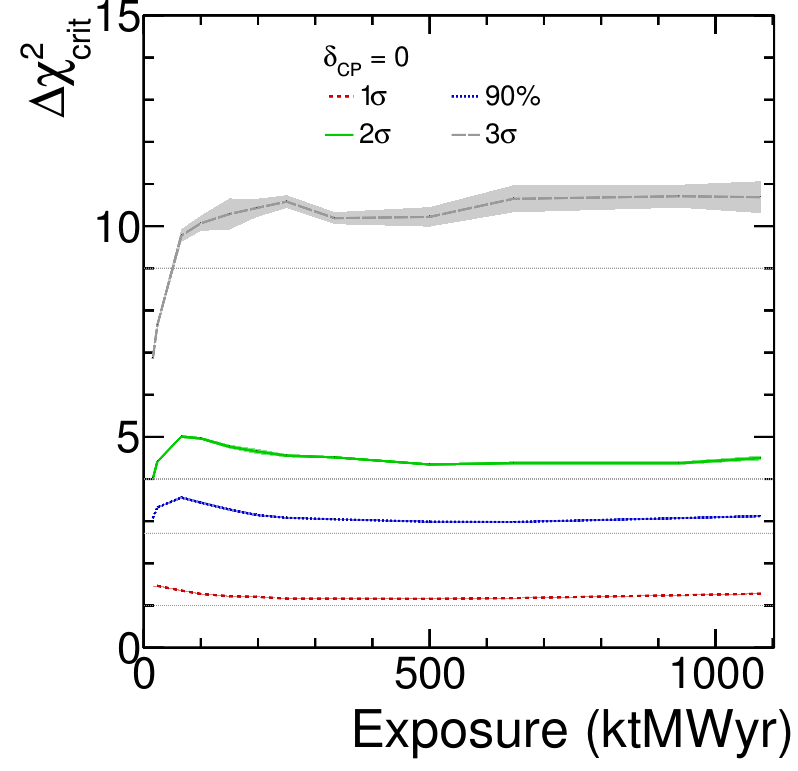
\includegraphics[width=0.8\columnwidth]{dchi2crit_vs_exp_dcp0.png}
  \caption{The \dchisqcrit values corresponding to 68.27\% (1$\sigma$), 90\%, 95.45\% (2$\sigma$) and 99.73\% (3$\sigma$) of throws, shown for true $\deltacp = 0$, as a function of exposure. The uncertainty on the \dchisqcrit values is obtained using Equation~\ref{eq:fc_uncertainty}, and is indicated as the shaded line. To guide the eye, horizontal dashed lines are included which indicate the 1$\sigma$, 90\%, 2$\sigma$ and 3$\sigma$ \dchisq values assumed using the constant-\dchisq method, with one degree of freedom. The distribution of throws used produced to calculate the \dchisqcrit values shown are given in Figure~\ref{fig:fc_throws_exp}.}
  \label{fig:fc_vs_exp}
\end{figure}
Figure~\ref{fig:fc_vs_exp} shows the evolution of the \dchisqcrit values as a function of exposure for $\deltacp = 0$, the relevant value for CPV sensitivity, for an ND+FD analysis with an equal FHC:RHC run fraction and a $\theta_{13}$ penalty applied. Several values were checked for $\deltacp = \pm\pi/2$ and similar results were found. The \dchisqcrit values for all significance levels tested rises quickly and stabilizes at slightly higher than than those suggested by the constant \dchisq method by exposures of $\sim$100 ktMWyr. The initial rise in the \dchisqcrit values is likely to be due to the low statistics at those exposures. Overall, this implies that the CPV significance is probably slightly weaker than assumed in, for example, Figures~\ref{fig:cpv_over_time} and~\ref{fig:cpv_vs_exp}, but not by a great deal. Crucially, there is no constant increase in the \dchisqcrit values over time as has been reported by T2K~\cite{Abe:2021gky}. Details on the number of toy throws used at each point of Figure~\ref{fig:fc_vs_exp} are given in Appendix~\ref{sec:fc_appendix}, and the toy throw distributions are shown in Figure~\ref{fig:fc_throws_exp}.

\begin{figure}[htbp]
  \centering
  \subfloat[100 ktMWyr]  {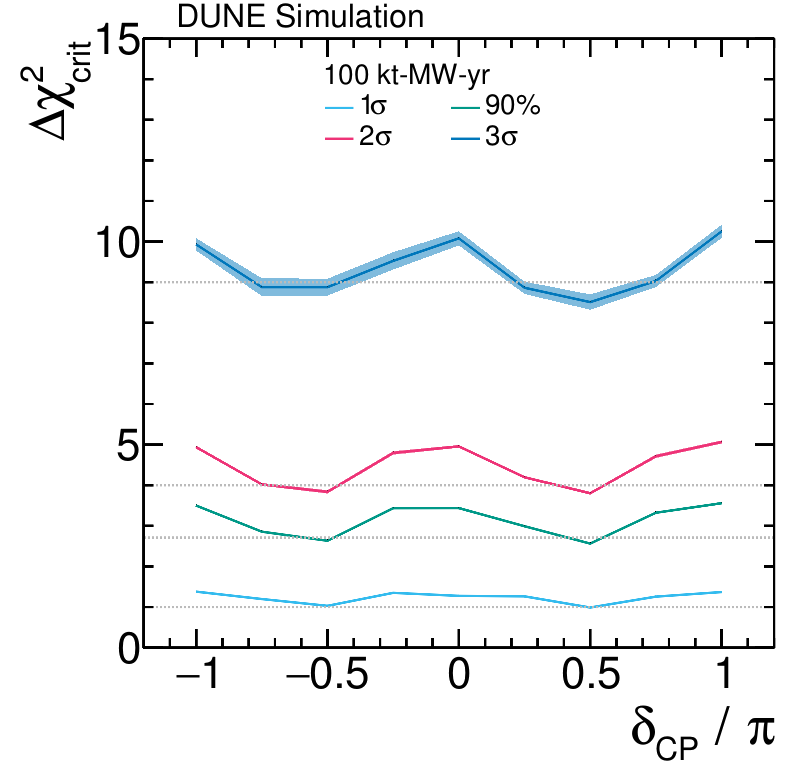
\includegraphics[width=0.8\columnwidth]{dchi2crit_vs_dcp_100ktMWyr.png}}\\
  \subfloat[334 ktMWyr]  {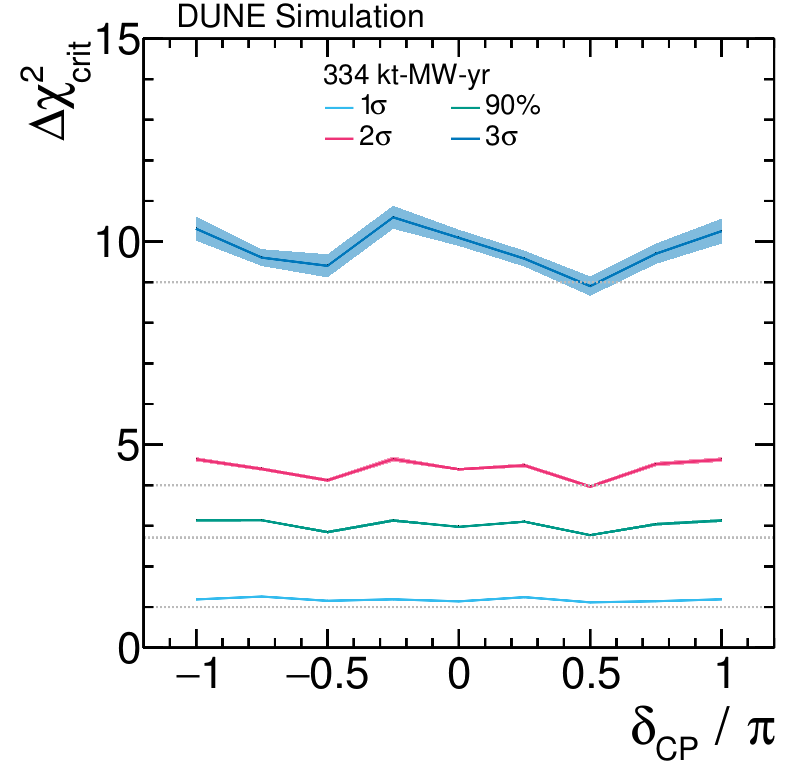
\includegraphics[width=0.8\columnwidth]{dchi2crit_vs_dcp_334ktMWyr.png}}
  \caption{The \dchisqcrit values corresponding to 68.27\% (1$\sigma$), 90\%, 95.45\% (2$\sigma$) and 99.73\% (3$\sigma$) of throws, shown as a function of true \deltacp, for exposures of 100 ktMWyr and 334 ktMWyr. The uncertainty on the \dchisqcrit values is obtained using Equation~\ref{eq:fc_uncertainty}, and is indicated as the shaded line. To guide the eye, horizontal dashed lines are included which indicate the 1$\sigma$, 90\%, 2$\sigma$ and 3$\sigma$ \dchisq values assumed using the constant-\dchisq method, with one degree of freedom. The distribution of throws used produced to calculate the \dchisqcrit values shown are given in Figure~\ref{fig:fc_throws_100ktMWyr} (Figure~\ref{fig:fc_throws_334ktMWyr}) for 100 ktMWyr (334 ktMWyr).}
  \label{fig:fc_vs_dcp}
\end{figure}
As \deltacp is a cyclical parameter, with physical boundaries at $\pm\pi$, it is interesting to see how the \dchisqcrit values evolve as a function of it. Figure~\ref{fig:fc_vs_dcp} shows the \dchisqcrit as a function of true \deltacp, for an ND+FD analysis with an equal FHC:RHC run fraction and a $\theta_{13}$ penalty applied, for 100 ktMWyr and 334 ktMWyr exposures. There is a noticeable, although not large, depression in the \dchisqcrit values at $\deltacp = \pm\pi/2$ for all significance levels considered. This effect is larger at the lower, 100 ktMWyr, exposure, and is larger at higher significance levels. It is also clear from Figure~\ref{fig:fc_vs_dcp} that the \dchisqcrit behaviour is very similar at $\delta = \pm\pi/2$ as at $\deltacp = 0$. Although the \dchisqcrit values are relevant for CPV sensitivity, this evolution of the \dchisqcrit values with \deltacp will be important for estimating DUNE's \deltacp resolution. Details on the number of toy throws used at each point of Figure~\ref{fig:fc_vs_dcp} are given in Appendix~\ref{sec:fc_appendix}, and the toy throw distributions are shown for the 100 ktMWyr (334 ktMWyr) test points in Figure~\ref{fig:fc_throws_100ktMWyr} (Figure~\ref{fig:fc_throws_334ktMWyr}).

\begin{figure*}[htbp]
  \centering
  \subfloat[24 ktMWyr]  {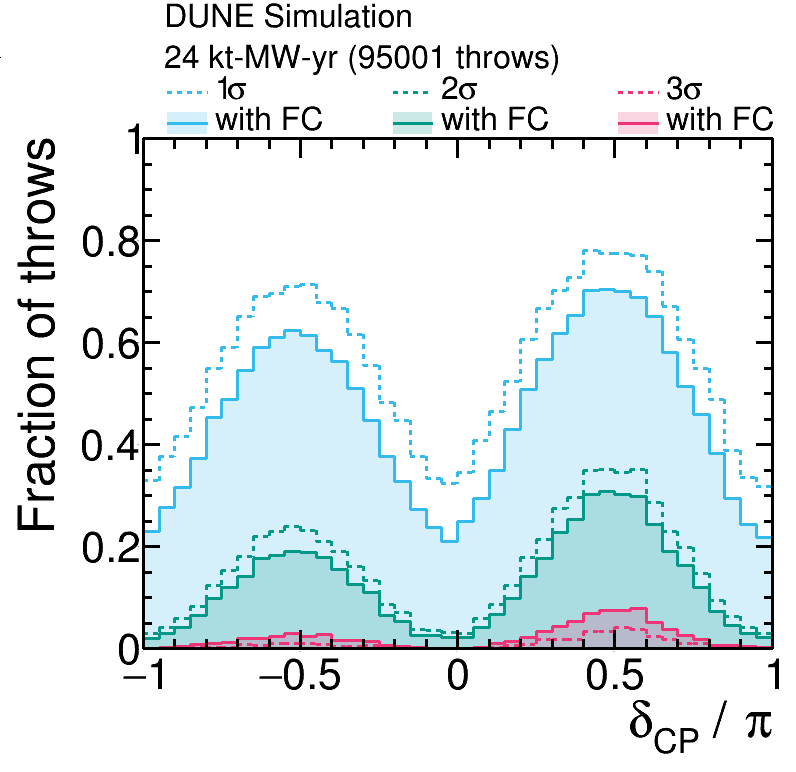
\includegraphics[width=0.33\linewidth]{cpv_throws_withFC_24ktMWyr_NH_th13.png}}
  \subfloat[66 ktMWyr]  {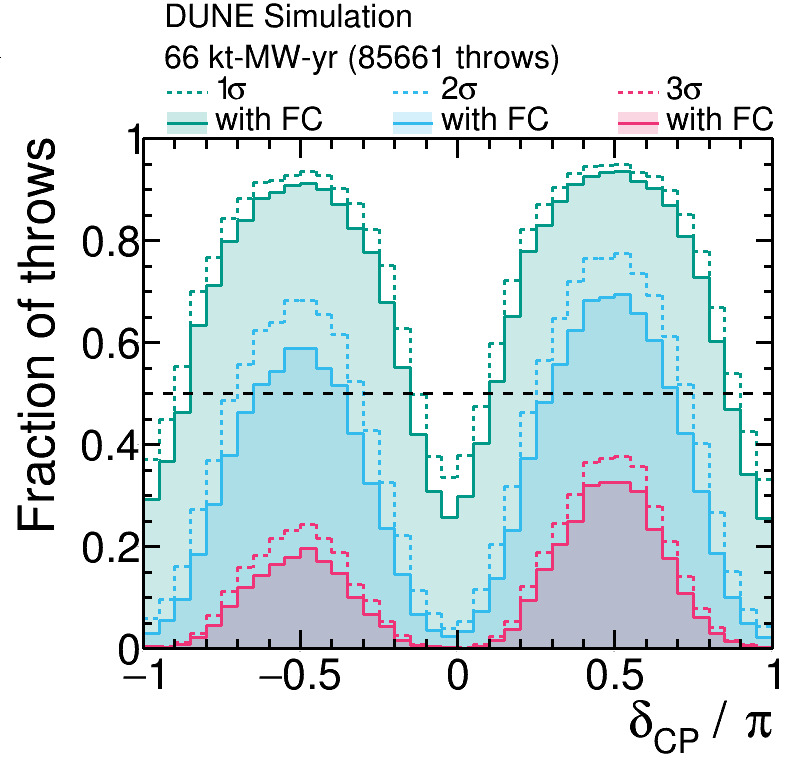
\includegraphics[width=0.33\linewidth]{cpv_throws_withFC_66ktMWyr_NH_th13.png}}
  \subfloat[100 ktMWyr] {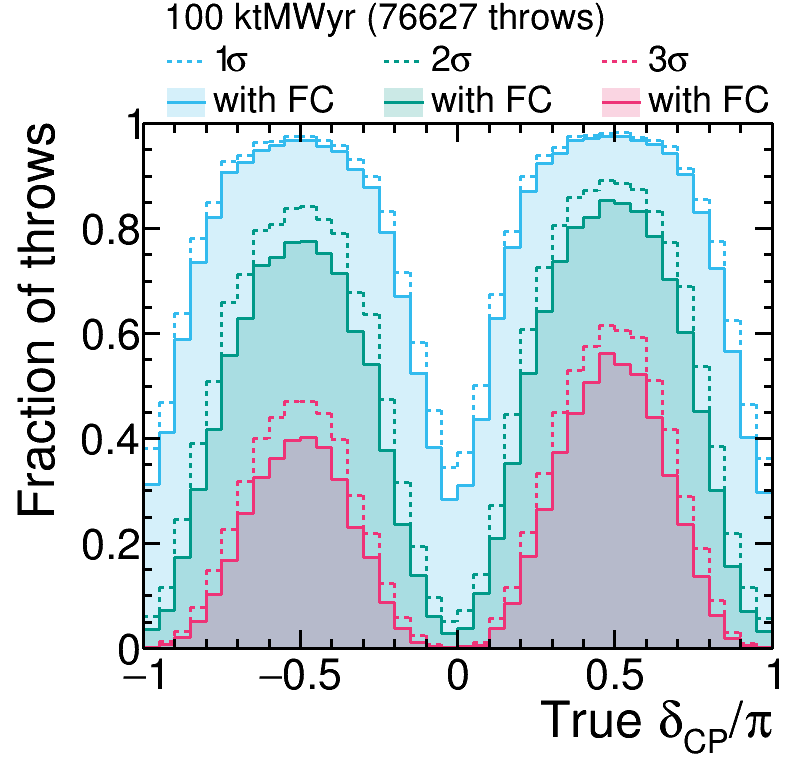
\includegraphics[width=0.33\linewidth]{cpv_throws_withFC_100ktMWyr_NH_th13.png}}\\
  \subfloat[150 ktMWyr] {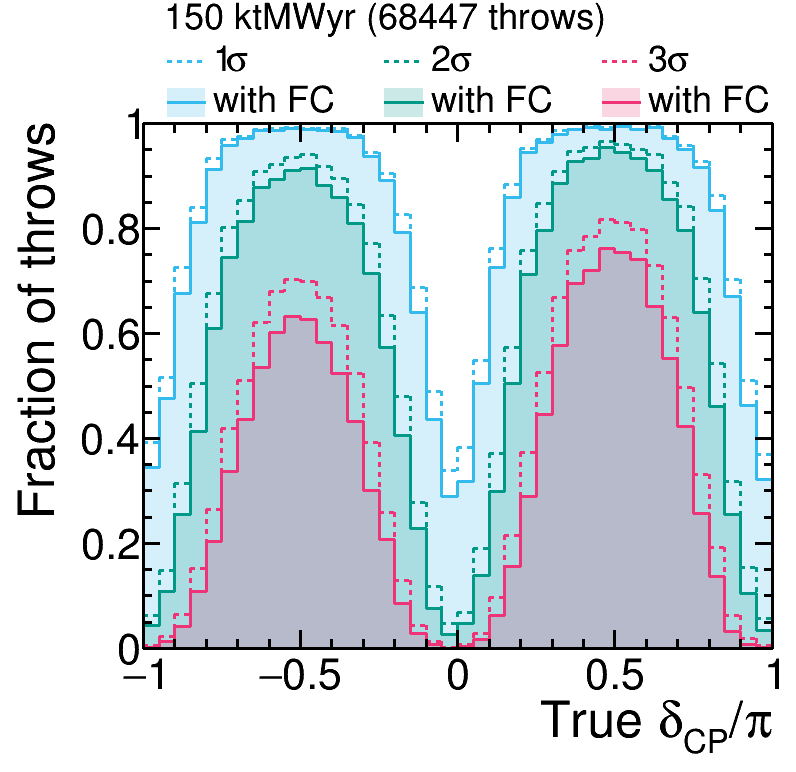
\includegraphics[width=0.33\linewidth]{cpv_throws_withFC_150ktMWyr_NH_th13.png}}
  \subfloat[197 ktMWyr] {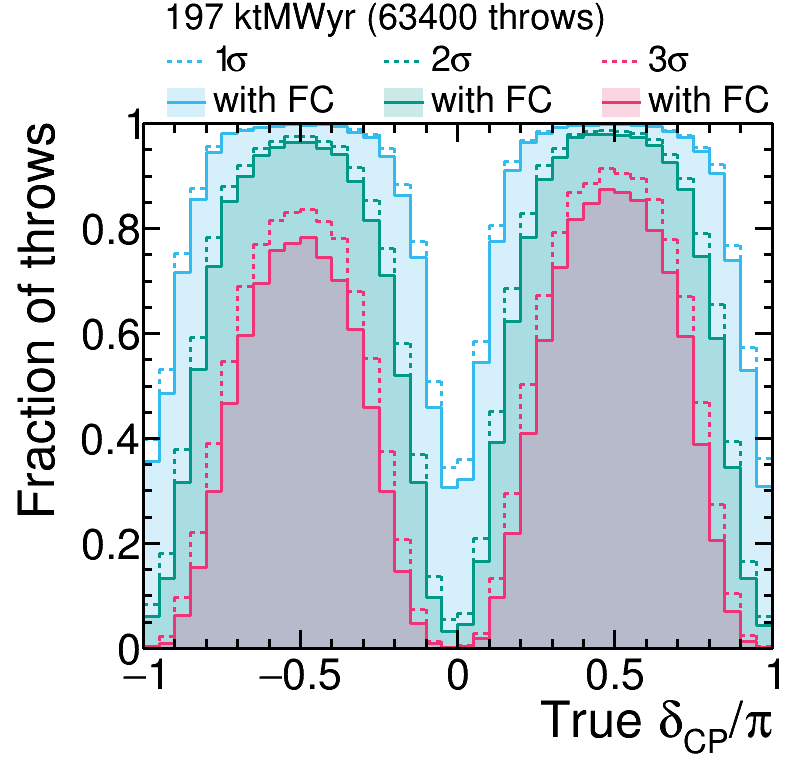
\includegraphics[width=0.33\linewidth]{cpv_throws_withFC_197ktMWyr_NH_th13.png}}
  \subfloat[334 ktMWyr] {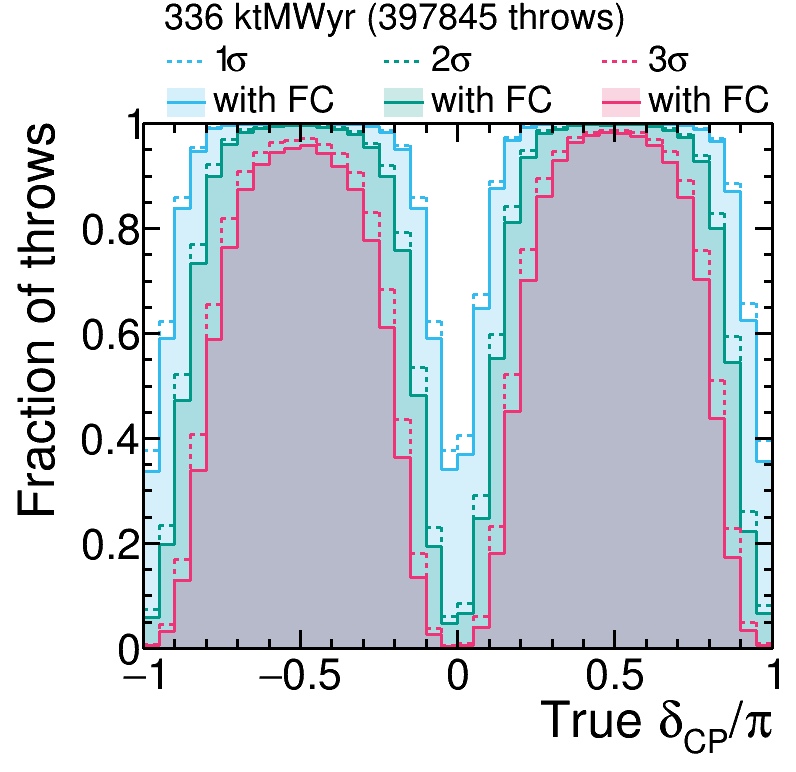
\includegraphics[width=0.33\linewidth]{cpv_throws_withFC_336ktMWyr_NH_th13.png}}
  \caption{Fraction of throws for which the DUNE sensitivity to CP-violation ($\deltacp \neq [0,\pm\pi]$) exceeds 1--3$\sigma$ significance, calculated using constant-\dchisq (dashed lines) and \dchisqcrit values calculated using the Feldman-Cousins method (shaded histograms), as a function of the true value of \deltacp. Shown for \dword{no}, for a number of different exposures. The number of throws used to make each figure is also shown.}
  \label{fig:cpv_over_time_fc}
\end{figure*}
Having calculated the \dchisqcrit values necessary to achieve correct coverage, it is possible to re-evaluate the CPV sensitivity previously shown assuming a constant \dchisq method in Figure~\ref{fig:cpv_over_time}. Figure~\ref{fig:cpv_over_time_fc} shows the 1, 2 and 3$\sigma$ CPV sensitivities as a function of true \deltacp, with and without the Feldman-Cousins correction (e.g., the \dchisqcrit values given in Figure~\ref{fig:fc_vs_exp} applied). The uncorrected values are the same as in Figure~\ref{fig:cpv_over_time}. In general, the effect of the Feldman-Cousins correction is to reduce the fraction of toy throws that cross each significance threshold, by a maximum of $\sim$10\%, but the eact fraction changes as a function of true \deltacp value and exposure. An exception to this general trend is the 3$\sigma$ behaviour at 24 ktMWyr, the lowest exposure shown, where the significance increases. This can be understood because of the rise in the 3$\sigma$ \dchisqcrit value at low exposures observed in Figure~\ref{fig:fc_vs_exp}.

\begin{figure*}[htbp]
  \centering
  \subfloat[$\deltacp = -\pi/2$] {\includegraphics[width=0.8\columnwidth]{{fraction_throws_vs_exp_dcp-0.5_FC}.pdf}}
  \subfloat[$\deltacp = +\pi/2$] {\includegraphics[width=0.8\columnwidth]{{fraction_throws_vs_exp_dcp0.5_FC}.pdf}}
  \caption{Fraction of throws for which the DUNE sensitivity to CP-violation ($\deltacp \neq [0,\pm\pi]$) exceeds 1--3$\sigma$ significance, at $\deltacp = \pm\pi/2$, calculated using constant-\dchisq (dashed lines) and \dchisqcrit values calculated using the Feldman-Cousins methed (shaded histograms), as a function of exposure.}
  \label{fig:cpv_vs_exp_fc}
\end{figure*}
Figure~\ref{fig:cpv_vs_exp_fc} shows the fraction of throws which exceed different significance thresholds at the maximal \deltacp violation values of $\pm\pi/2$, as a function of exposure, with and without Feldman-Cousins corrections, for 1--3$sigma$ significance values. It is clear from Figure~\ref{fig:cpv_vs_exp_fc} that the effect of the correction is not large, and $\sim$10\% longer exposures are required for the median sensitivity to cross each significance threshold than without correction, at both points shown.

\FloatBarrier
